\chapter{Proposed Methodology}
\label{ch:methodology}

\section{System Architecture and Control Pipeline}
The autonomous intersection decision-making pipeline operates across two coupled layers: the microscopic multi-agent traffic simulator (SUMO interfaced via UC Berkeley Flow) and the DRL agent (\autoref{fig:pomdp_pipeline}). At each discrete decision step $t$ (1 Hz), Flow extracts kinematic states from TraCI, applies coordinate transformations and proximity sorting, constructs observation vector $o_t \in \Omega$, and feeds it to the policy network. The actor selects discrete action $a_t \in \mathcal{A}$ modulating target velocity $v_{\text{tar}}$. A lower-level proportional controller commands continuous acceleration $a_{\text{cmd}}$ across 15 simulation substeps (15 Hz).

\vspace{-0.2cm}
\begin{figure}[htbp]
    \centering
    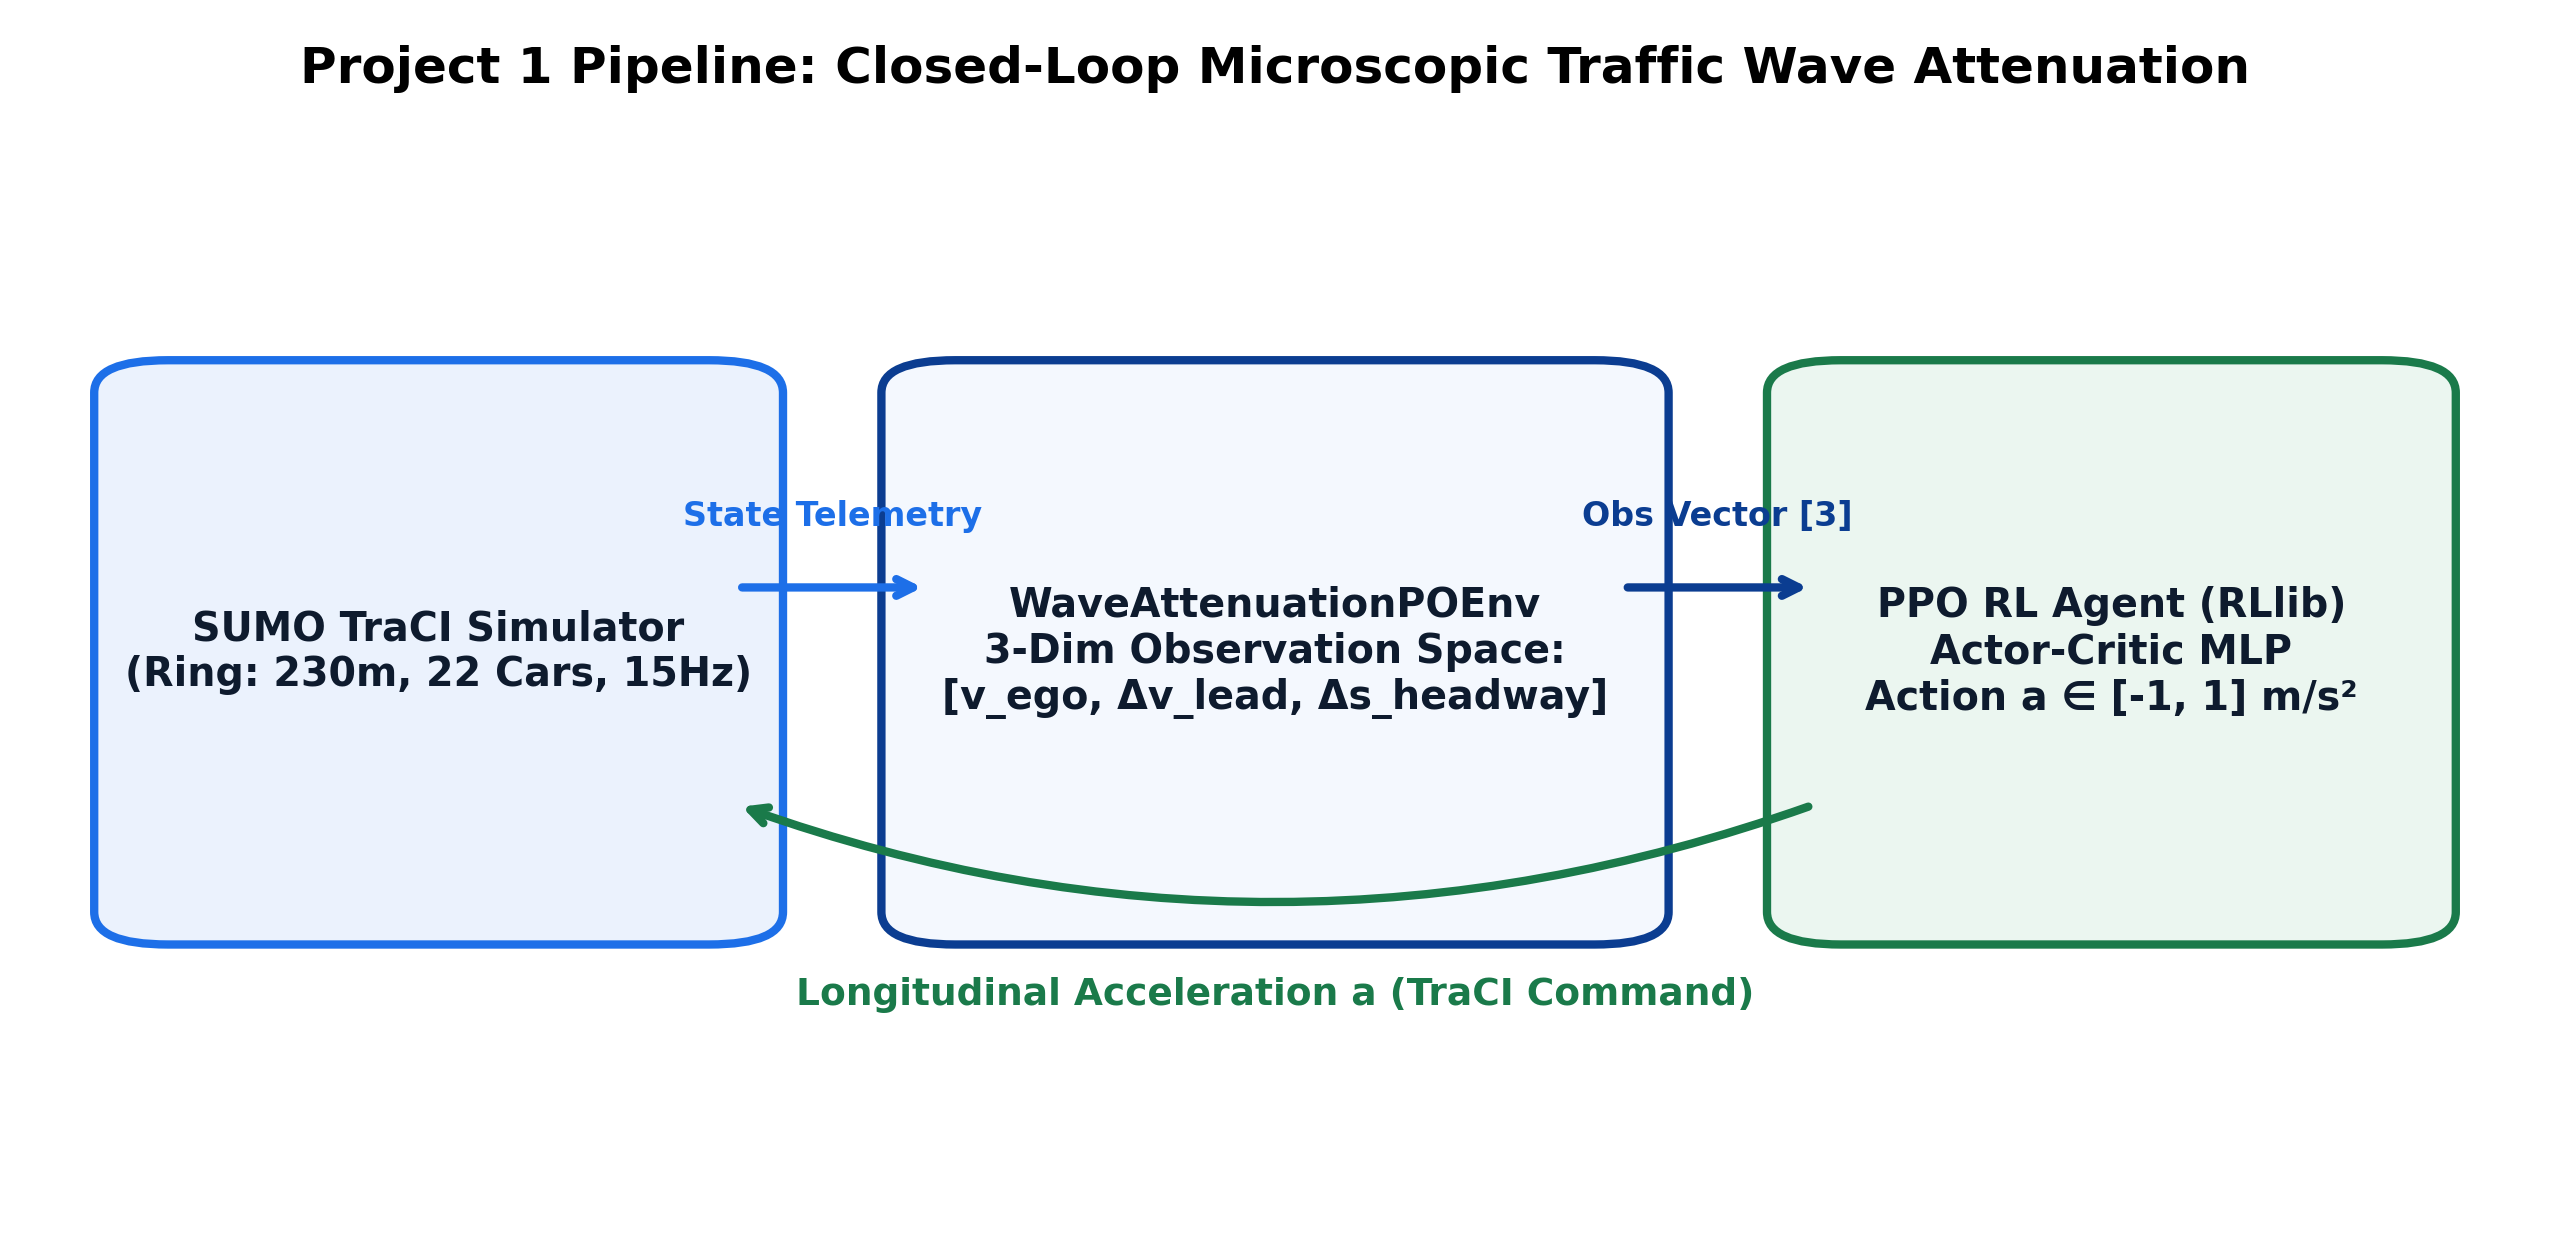
\includegraphics[width=0.78\textwidth, height=2.6cm, keepaspectratio]{figures/ring_pomdp_pipeline.png}
    \vspace{-0.2cm}
    \caption{Closed-Loop System Architecture and POMDP Control Pipeline linking TraCI/SUMO to Actor-Critic Policies.}
    \label{fig:pomdp_pipeline}
\end{figure}

\vspace{-0.2cm}
\section{Observation State Space Formulations}
Both configurations monitor the autonomous ego vehicle (AEV) and up to $N = 9$ surrounding vehicles within radar radius $R_{\text{detect}} = 48.0$ m (zero-padded if $<9$), sorted by Euclidean distance $d_i = \sqrt{(x_i - x_{\text{ego}})^2 + (y_i - y_{\text{ego}})^2} \le 48.0$ m. Each vehicle $i \in \{1, \dots, 9\}$ contributes a 6-dim relative observation vector:
\begin{equation}
    S_i = [p_i, \; \Delta x_i, \; \Delta y_i, \; \Delta v_{x,i}, \; \Delta v_{y,i}, \; \phi_i] \in \mathbb{R}^6
\end{equation}
where $p_i \in \{0, 1\}$ is existence, $\Delta x_i, \Delta y_i$ are relative offsets, $\Delta v_{x,i}, \Delta v_{y,i}$ are relative velocities, and $\phi_i$ is heading.

\subsection{Config Original (Baseline, 60-Dimensional State)}
The baseline ego state encompasses purely kinematic quantities without destination awareness:
\begin{equation}
    S_{\text{ego}}^{\text{Orig}} = [p_{\text{ego}}, \; x_{\text{ego}}, \; y_{\text{ego}}, \; v_{x,\text{ego}}, \; v_{y,\text{ego}}, \; \phi_{\text{ego}}] \in \mathbb{R}^6, \quad S_{\text{total}}^{\text{Orig}} = [S_{\text{ego}}^{\text{Orig}}, S_1, \dots, S_9] \in \mathbb{R}^{60}
\end{equation}

\subsection{Config B (Task-Intent Augmented, 61-Dimensional State)}
Config B incorporates task-intent feature $\mu_a$ \cite{xiao2024decision}, expanding the ego slot to 7 dimensions:
\begin{equation}
    S_{\text{ego}}^{B} = [p_{\text{ego}}, \; x_{\text{ego}}, \; y_{\text{ego}}, \; v_{x,\text{ego}}, \; v_{y,\text{ego}}, \; \phi_{\text{ego}}, \; \mu_a] \in \mathbb{R}^7, \quad S_{\text{total}}^{B} = [S_{\text{ego}}^{B}, S_1, \dots, S_9] \in \mathbb{R}^{61}
\end{equation}
The driving intent parameter $\mu_a$ encodes task completion and directional orientation toward the exit node:
\begin{equation}
    \mu_a = \begin{cases}
        \arctan\left(d_a / d_{\text{total}}\right) & \text{if task is Straight Crossing} \\
        |\phi_{\text{ego}} - \theta_a| & \text{if task is Left Turn or Right Turn}
    \end{cases}
    \label{eq:mu_a}
\end{equation}
where $d_a$ is remaining distance to exit, $d_{\text{total}}$ is total crossing length, and $\theta_a$ is bearing to exit. Normalization ensures $\mu_a \approx \pi/4$ at entry, smoothly decaying to zero upon task completion.

\vspace{-0.2cm}
\section{Action Mapping and Proportional Controller}
Action $a_t \in \{0: \text{Accelerate (+1)}, 1: \text{Idle (0)}, 2: \text{Decelerate (-1)}\}$ modulates target speed $v_{\text{tar}} \in \{0, \dots, 8\}$ m/s via $v_{\text{dis}} = \text{round}(v_{\text{actual}})$. Acceleration is commanded via proportional control: $a_{\text{cmd}} = K_P \cdot (v_{\text{tar}} - v_{\text{actual}})$ with $K_P = 5.0\text{ s}^{-1}$, guaranteeing rapid speed convergence within the 1-second policy step.

\vspace{-0.2cm}
\section{Comparative Evaluation of State-of-the-Art RL Algorithms}
\label{sec:algo_comparison}
To address Washington Accord criteria, three RL algorithm families were evaluated (\autoref{tab:algo_comparison}).

\begin{table}[htbp]
\centering
\footnotesize
\renewcommand{\arraystretch}{0.95}
\resizebox{\textwidth}{!}{%
\begin{tabular}{|l|p{3.5cm}|p{3.5cm}|p{3.8cm}|}
\hline
\textbf{Criteria} & \textbf{PPO (On-Policy)} & \textbf{DQN (Value-Based)} & \textbf{Discrete SAC (Max-Entropy)} \\ \hline
\textbf{Sample Efficiency} & Low: Requires $>10^6$ transitions. & High: Reuses replay buffer. & \textbf{Highest}: Off-policy soft policy iteration. \\ \hline
\textbf{Exploration} & Logit entropy penalty; early collapse. & $\epsilon$-greedy random exploration. & \textbf{Entropy-Maximizing}: Auto-tuned $\alpha$. \\ \hline
\textbf{Action Alignment} & High gradient variance under sparse reward. & Q-value overestimation bias. & \textbf{Twin Q-Networks}: Mitigates bias. \\ \hline
\textbf{Convergence} & Stable surrogate, but slow creeping. & Prone to divergence in multi-agent. & \textbf{Highly Stable}: Twin critics, Polyak $\tau=0.005$. \\ \hline
\end{tabular}%
}
\vspace{-0.2cm}
\caption{Comparative Multi-Criteria Decision Analysis of Reinforcement Learning Algorithms}
\label{tab:algo_comparison}
\end{table}

\textbf{Selection Rationale}: \textbf{Discrete Soft Actor-Critic (SAC)} was selected for the exact reproduction (Phase 2) due to: (i) \textit{Sample Efficiency} (converging in 50k episodes vs. 1.2M for PPO); (ii) \textit{Entropy Exploration} preventing creeping policies; and (iii) \textit{Twin Critic Estimation} mitigating value overestimation.

